\chapter{Introduction}

Natural language processing (NLP) is a subfield of linguistics, computer science, and artificial intelligence dealing with the interaction between computers and humans using natural language. NLPs main objective is to decipher, interpret, and react to human language which often relies on machine learning (ML) techniques. Natural language includes both speech and text \cite{garbade}. There exist many use cases for NLP such as text-to-speech transformation, machine translation\footnote{Translating one written language into another like Google Translator or DeepL does}, part-of-speech tagging\footnote{The process of identifying nouns, verbs, adjectives, adverbs, etc.}, and named-entity recognition. This bachelor thesis is about the latter topic, also called NER.

\section{Project Overview}

Mobi24 is an assistance and emergency call centre founded by the Swiss Mobiliar in 1997. It's the initial contact point for clients and potential future clients. Most of the in-going requests are insurance related subjects. The purpose of this bachelor thesis is the creation of a natural language model for named-entity recognition in the insurance context based on client data from Mobi24. There already exist several pretrained models which are free to use, but just a few of them are capable of dealing with the German language and none of them are trained with insurance data. In the future, the model from this thesis should help the data scientists at Swiss Mobiliar for their own specific NLP tasks. Currently the most interesting named entities for Swiss Mobiliar are the people's names and their addresses. Consider chapter \ref{chap:ner-overview} for detailed information about NER and how it works.

\subsection{Objectives}

For a successful completion of the bachelor thesis several deliverables need to be offered to the stakeholders. Additionally to this document there should exist a functioning language model with an anonymised test data set. This data set should have an appropriate size for evaluating the model's performance. The source code should be written under consideration of the commonly known software engineering and design patterns. The model is developed iteratively with one or more baseline models\footnote{A very simple approach which sets the minimal requirements for NER} at beginning. The goal is to optimise the model with every new approach to get the most accurate output possible.

From an administrative point of view there are several deliverables this bachelor thesis has to provide. A summarized overview about all objectives can be found in the table below. Consider table \ref{tbl:deadlines} for the corresponding deadlines.

\begin{enumerate}
    \item NER model (with anonymised test data)
    \item Bachelor thesis (current document)
    \item Presentation for the BFH techdays 2020
    \item Abstract for the BFH publication of all bachelor theses
    \item Poster (of size A3)
    \item Short movie clip about the project's essentials
\end{enumerate}

\subsection{Submission Deadlines}

This bachelor thesis is carried out in compliance with various deadlines. Table \ref{tbl:deadlines} gives an insight about the most relevant milestones and when they should be delivered to the stakeholders.

\begin{table}[ht!]
    \centering
    \begin{tabular}{|l|l|}
        \hline
        \textbf{Date} & \textbf{Submissions and Milestones} \\ [0.5ex]
        \hline
        16.09.2019 & Begin of semester, project kick off \\
        03.01.2020 & Submission of poster (A3) \\
        16.01.2020 & Submission of report, movie clip \\
        17.01.2020 & Presentation at BFH Techday \\
        17.01.2020 & Poster exhibition \\
        07.02.2020 & Grading conference \\
        06.03.2020 & Graduation party \\ [1ex]
        \hline
    \end{tabular}
    \caption{Most important (submission) dates}
    \label{tbl:deadlines}
\end{table}

\subsection{Stakeholders}

There are several stakeholders interested in the outcome of this project. There is the Swiss Mobiliar and especially its data scientists, who want to reuse the trained NLP model for their own projects. On the other hand, there is the Bern University of Applied Sciences (BFH) which is demanding a satisfactory thesis for awarding me with the bachelor's degree in computer science. Last but not least, I act as a stakeholder as well and I want to dig deeper in the field of data science and learn as much as possible.

It will be challenging to satisfy all these different stakeholders to an adequate level. Swiss Mobiliar is very focused on the resulting model whereas the BFH is more interested in the overall project, including time and project management.

\section{Organisation}

This bachelor thesis is written during my last semester at the Bern University of Applied Sciences while I'm working full-time at the Swiss Mobiliar in the Department of \emph{Cognitive Computing \& Disruptive Analytics}. The department is mainly responsible for the development of cognitive applications to support existing business processes. The team is also driving the digital transformation and making Swiss Mobiliar data addicted.

\subsection{Coordination}

Swiss Mobiliar is working with the \emph{Atlassian} tool stack. \emph{Jira} is used for keeping track of all tasks and dealing with bug requests. The Kanban boards model the current project state by visualising the progress of each story or task.

I'm a member of the agile Scrum team \emph{Aare}\footnote{The beautiful river called Aare floats through the city of Berne}. Due to the Scrum methodology, my colleagues are getting informed about my progress every morning at the daily scrum. At the end of each sprint\footnote{At Swiss Mobiliar a sprint has a total duration of 3 weeks}, there is a Scrum activity called \emph{Sprint Review} where I present my latest findings to the team.

\begin{figure}[!ht]
\centering
\frame{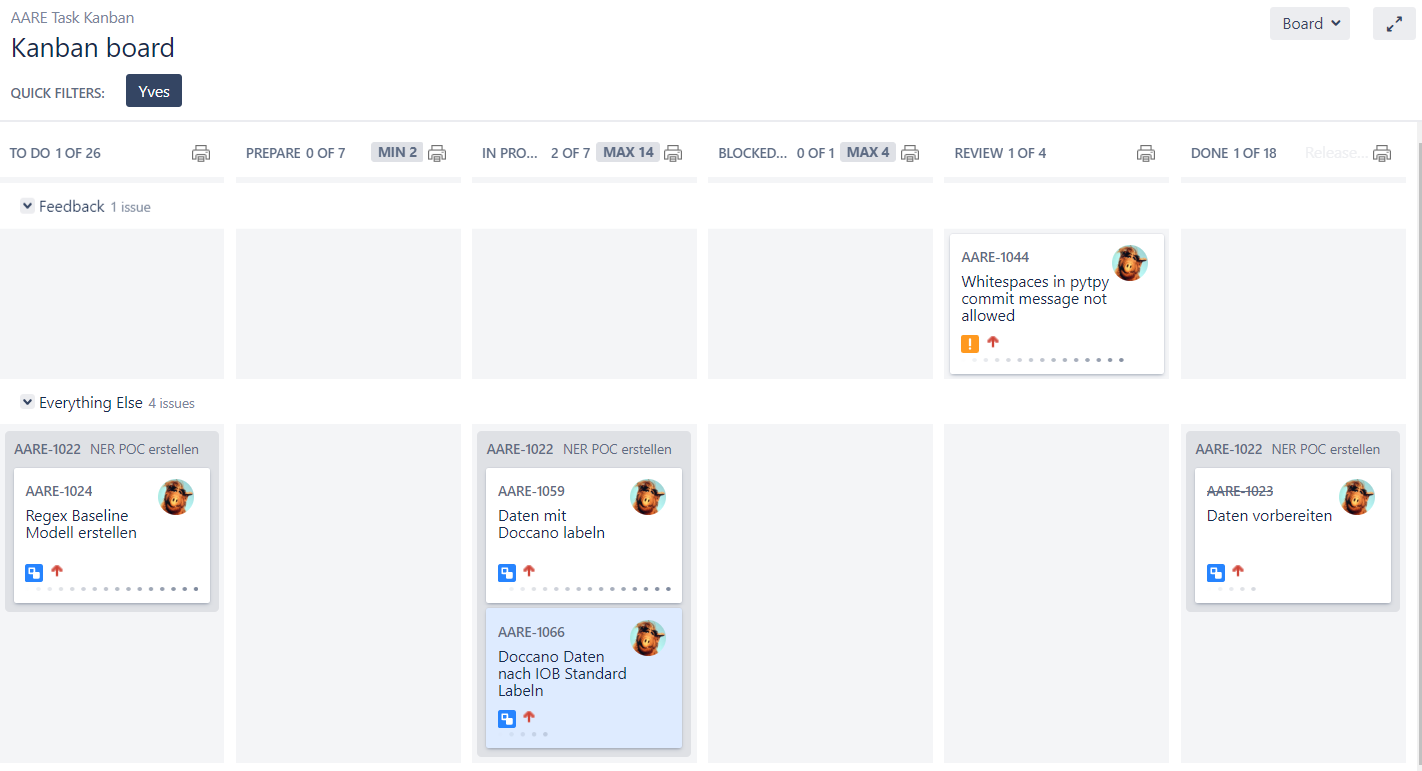
\includegraphics[width=\textwidth]{kanban}}
\caption{View of the Kanban board at an early project stage}
\label{fig:kanban}
\end{figure}

My supervising professor and I organise an informal meeting roughly every two weeks to discuss the project progress and to plan the next steps. During this session I've got the time to ask questions concerning my current tasks. Due to the short time span between these meetings, the project itself becomes very agile. I am able to change my primary focus to a different task within weeks.

\subsection{Development Environment}

All source code is generally written in Python. Small code snippets, mostly for exploring and mapping data into another structure, are created with \emph{jupyter notebooks}. The models and larger pre-processing steps need to be robust and comprehensible, so unit tests must be created. This code is under version control and is pushed frequently to the internal Git repository of Swiss Mobiliar. Teamcity is used as a build server, which controls and deploys the code as a python library. To simulate later applications, the model code is being run inside a docker container\footnote{Tool to run applications inside a container independent of the underlying operating system}.

\section{Data Privacy Declaration}

All used examples and data snippets in this document are anonymised to protect the privacy of Swiss Mobiliar's clients. All names and addresses are either cropped out of the original text or purely fictional. The test data given to the supervising professor for validating the final model is anonymised too.
